% Copyright © 2012-2013 Martin Ueding <dev@martin-ueding.de>

% This is my general purpose LaTeX header file for writing German documents.
% Ideally, you include this using a simple ``% Copyright © 2012-2013 Martin Ueding <dev@martin-ueding.de>

% This is my general purpose LaTeX header file for writing German documents.
% Ideally, you include this using a simple ``% Copyright © 2012-2013 Martin Ueding <dev@martin-ueding.de>

% This is my general purpose LaTeX header file for writing German documents.
% Ideally, you include this using a simple ``\input{header.tex}`` in your main
% document and start with ``\title`` and ``\begin{document}`` afterwards.

% If you need to add additional packages, I recommend not doing this in this
% file, but in your main document. That way, you can just drop in a new
% ``header.tex`` and get all the new commands without having to merge manually.

% Since this file encorporates a CC-BY-SA fragment, this whole files is
% licensed under the CC-BY-SA license.

\documentclass[11pt, ngerman, fleqn, DIV=15, headinclude]{scrartcl}

\usepackage{graphicx}

\setkomafont{caption}{\sffamily}
\setkomafont{captionlabel}{\usekomafont{caption}}

%%%%%%%%%%%%%%%%%%%%%%%%%%%%%%%%%%%%%%%%%%%%%%%%%%%%%%%%%%%%%%%%%%%%%%%%%%%%%%%
%                                Locale, date                                 %
%%%%%%%%%%%%%%%%%%%%%%%%%%%%%%%%%%%%%%%%%%%%%%%%%%%%%%%%%%%%%%%%%%%%%%%%%%%%%%%

\usepackage{babel}
\usepackage[iso]{isodate}

%%%%%%%%%%%%%%%%%%%%%%%%%%%%%%%%%%%%%%%%%%%%%%%%%%%%%%%%%%%%%%%%%%%%%%%%%%%%%%%
%                          Margins and other spacing                          %
%%%%%%%%%%%%%%%%%%%%%%%%%%%%%%%%%%%%%%%%%%%%%%%%%%%%%%%%%%%%%%%%%%%%%%%%%%%%%%%

\usepackage[parfill]{parskip}
\usepackage{setspace}
\usepackage[activate]{microtype}

\setlength{\columnsep}{2cm}

%%%%%%%%%%%%%%%%%%%%%%%%%%%%%%%%%%%%%%%%%%%%%%%%%%%%%%%%%%%%%%%%%%%%%%%%%%%%%%%
%                                    Color                                    %
%%%%%%%%%%%%%%%%%%%%%%%%%%%%%%%%%%%%%%%%%%%%%%%%%%%%%%%%%%%%%%%%%%%%%%%%%%%%%%%

\usepackage[usenames, dvipsnames]{xcolor}

\colorlet{darkred}{red!70!black}
\colorlet{darkblue}{blue!70!black}
\colorlet{darkgreen}{green!40!black}

%%%%%%%%%%%%%%%%%%%%%%%%%%%%%%%%%%%%%%%%%%%%%%%%%%%%%%%%%%%%%%%%%%%%%%%%%%%%%%%
%                         Font and font like settings                         %
%%%%%%%%%%%%%%%%%%%%%%%%%%%%%%%%%%%%%%%%%%%%%%%%%%%%%%%%%%%%%%%%%%%%%%%%%%%%%%%

% This replaces all fonts with Bitstream Charter, Bitstream Vera Sans and
% Bitstream Vera Mono. Math will be rendered in Charter.
\usepackage[charter, greekuppercase=italicized]{mathdesign}
\usepackage{beramono}
\usepackage{berasans}

% Bold, sans-serif tensors. This fragment is taken from “egreg” from
% http://tex.stackexchange.com/a/82747/8945 and licensed under `CC-BY-SA
% <https://creativecommons.org/licenses/by-sa/3.0/>`_.
\usepackage{bm}
\DeclareMathAlphabet{\mathsfit}{\encodingdefault}{\sfdefault}{m}{sl}
\SetMathAlphabet{\mathsfit}{bold}{\encodingdefault}{\sfdefault}{bx}{sl}
\newcommand{\tens}[1]{\bm{\mathsfit{#1}}}

% Bold vectors.
\renewcommand{\vec}[1]{\boldsymbol{#1}}

%%%%%%%%%%%%%%%%%%%%%%%%%%%%%%%%%%%%%%%%%%%%%%%%%%%%%%%%%%%%%%%%%%%%%%%%%%%%%%%
%                               Input encoding                                %
%%%%%%%%%%%%%%%%%%%%%%%%%%%%%%%%%%%%%%%%%%%%%%%%%%%%%%%%%%%%%%%%%%%%%%%%%%%%%%%

\usepackage[T1]{fontenc}
\usepackage[utf8]{inputenc}

%%%%%%%%%%%%%%%%%%%%%%%%%%%%%%%%%%%%%%%%%%%%%%%%%%%%%%%%%%%%%%%%%%%%%%%%%%%%%%%
%                         Hyperrefs and PDF metadata                          %
%%%%%%%%%%%%%%%%%%%%%%%%%%%%%%%%%%%%%%%%%%%%%%%%%%%%%%%%%%%%%%%%%%%%%%%%%%%%%%%

\usepackage{hyperref}

% This sets the author in the properties of the PDF as well. If you want to
% change it, just override it with another ``\hypersetup`` call.
\hypersetup{
	breaklinks=false,
	citecolor=darkgreen,
	colorlinks=true,
	linkcolor=darkblue,
	menucolor=black,
	pdfauthor={Martin Ueding},
	urlcolor=darkblue,
}

%%%%%%%%%%%%%%%%%%%%%%%%%%%%%%%%%%%%%%%%%%%%%%%%%%%%%%%%%%%%%%%%%%%%%%%%%%%%%%%
%                               Math Operators                                %
%%%%%%%%%%%%%%%%%%%%%%%%%%%%%%%%%%%%%%%%%%%%%%%%%%%%%%%%%%%%%%%%%%%%%%%%%%%%%%%

% AMS environments like ``align`` and theorems like ``proof``.
\usepackage{amsmath}
\usepackage{amsthm}

% Common math constructs like partial derivatives.
\usepackage{commath}

% Physical units.
\usepackage[output-decimal-marker={,}]{siunitx}

% Since I use mathdesign with italic uppercase greek characters, the Ohm unit will be displayed with an italic Ω by default. Units have to be roman, so this forces it the right way.
\DeclareSIUnit{\ohm}{$\Omegaup$}
\DeclareSIUnit{\division}{DIV}
\DeclareSIUnit{\voltss}{$\mathrm{V_{SS}}$}

% Word like operators.
\DeclareMathOperator{\acosh}{arcosh}
\DeclareMathOperator{\arcosh}{arcosh}
\DeclareMathOperator{\arcsinh}{arsinh}
\DeclareMathOperator{\arsinh}{arsinh}
\DeclareMathOperator{\asinh}{arsinh}
\DeclareMathOperator{\card}{card}
\DeclareMathOperator{\csch}{csch}
\DeclareMathOperator{\diam}{diam}
\DeclareMathOperator{\sech}{sech}
\renewcommand{\Im}{\mathop{{}\mathrm{Im}}\nolimits}
\renewcommand{\Re}{\mathop{{}\mathrm{Re}}\nolimits}

% Fourier transform.
\DeclareMathOperator{\fourier}{\ensuremath{\mathcal{F}}}

% Roman versions of “e” and “i” to serve as Euler's number and the imaginary
% constant.
\newcommand{\eup}{\mathrm e}
\newcommand{\iup}{\mathrm i}

% Symbols for the various mathematical fields (natural numbers, integers,
% rational numbers, real numbers, complex numbers).
\newcommand{\C}{\ensuremath{\mathbb C}}
\newcommand{\N}{\ensuremath{\mathbb N}}
\newcommand{\Q}{\ensuremath{\mathbb Q}}
\newcommand{\R}{\ensuremath{\mathbb R}}
\newcommand{\Z}{\ensuremath{\mathbb Z}}

% Shape like operators.
\DeclareMathOperator{\dalambert}{\Box}
\DeclareMathOperator{\laplace}{\bigtriangleup}
\newcommand{\curl}{\vnabla \times}
\newcommand{\divergence}[1]{\inner{\vnabla}{#1}}
\newcommand{\Divergence}[1]{\Inner{\vnabla}{#1}}
\newcommand{\vnabla}{\vec \nabla}

\newcommand{\half}{\frac 12}

% Unit vector (German „Einheitsvektor“).
\newcommand{\ev}{\hat{\vec e}}

% Mathematician's notation for the inner (scalar, dot) product.
\newcommand{\bracket}[1]{\langle #1 \rangle}
\newcommand{\Bracket}[1]{\left\langle #1 \right\rangle}
\newcommand{\inner}[2]{\bracket{#1, #2}}
\newcommand{\Inner}[2]{\Bracket{#1, #2}}

% Placeholders.
\newcommand{\fehlt}{\textcolor{darkred}{Hier fehlen noch Inhalte.}}
\newcommand{\messwert}{\textcolor{blue}{\square}}
\newcommand{\punkte}{\phantom{xxxxx}}

% Separator for equations on a single line.
\newcommand{\eqnsep}{,\quad}

% Quantum Mechanics.
\usepackage{braket}

% Thermodynamic partial derivative.
\newcommand\tdpd[3]{\del{\dpd{#1}{#2}}_{#3}}

%%%%%%%%%%%%%%%%%%%%%%%%%%%%%%%%%%%%%%%%%%%%%%%%%%%%%%%%%%%%%%%%%%%%%%%%%%%%%%%
%                                  Headings                                   %
%%%%%%%%%%%%%%%%%%%%%%%%%%%%%%%%%%%%%%%%%%%%%%%%%%%%%%%%%%%%%%%%%%%%%%%%%%%%%%%

% This will set fancy headings to the top of the page. The page number will be
% accompanied by the total number of pages. That way, you will know if any page
% is missing.
%
% If you do not want this for your document, you can just use
% ``\pagestyle{plain}``.

\usepackage{scrpage2}

\pagestyle{scrheadings}
\automark{section}
\chead{}
\ihead{}
\ohead{\rightmark}
\setheadsepline{.4pt}

%%%%%%%%%%%%%%%%%%%%%%%%%%%%%%%%%%%%%%%%%%%%%%%%%%%%%%%%%%%%%%%%%%%%%%%%%%%%%%%
%                            Bibliography (BibTeX)                            %
%%%%%%%%%%%%%%%%%%%%%%%%%%%%%%%%%%%%%%%%%%%%%%%%%%%%%%%%%%%%%%%%%%%%%%%%%%%%%%%

\newcommand{\bibliographyfile}{../../zentrale_BibTeX/Central}

\usepackage[
    backend=bibtex,
    style=authoryear-icomp,
    %isbn=false,
    %pagetracker=false,
    %maxbibnames=50,
    %maxcitenames=2,
    %autocite=inline,
    %block=space,
    %backref=false,
    %backrefstyle=three+,
    %date=short,
    hyperref=true
]{biblatex}

\setlength{\bibitemsep}{.7em}
\setlength{\bibhang}{4ex}

\IfFileExists{\bibliographyfile}{
    \bibliography{\bibliographyfile}
}{}

%%%%%%%%%%%%%%%%%%%%%%%%%%%%%%%%%%%%%%%%%%%%%%%%%%%%%%%%%%%%%%%%%%%%%%%%%%%%%%%
%                                Abbreviations                                %
%%%%%%%%%%%%%%%%%%%%%%%%%%%%%%%%%%%%%%%%%%%%%%%%%%%%%%%%%%%%%%%%%%%%%%%%%%%%%%%

\newcommand{\dhabk}{\mbox{d.\,h.}}

%%%%%%%%%%%%%%%%%%%%%%%%%%%%%%%%%%%%%%%%%%%%%%%%%%%%%%%%%%%%%%%%%%%%%%%%%%%%%%%
%                                  Licences                                   %
%%%%%%%%%%%%%%%%%%%%%%%%%%%%%%%%%%%%%%%%%%%%%%%%%%%%%%%%%%%%%%%%%%%%%%%%%%%%%%%

\usepackage{ccicons}

\newcommand{\ccbysadetext}{%
	\begin{small}
		Dieses Werk bzw. Inhalt steht unter einer
		\href{http://creativecommons.org/licenses/by-sa/3.0/deed.de}{%
			Creative Commons Namensnennung - Weitergabe unter gleichen
		Bedingungen 3.0 Unported Lizenz}.
	\end{small}
}

\newcommand{\ccbysadetitle}{%
	Lizenz: \href{http://creativecommons.org/licenses/by-sa/3.0/deed.de}
	{CC-BY-SA 3.0 \ccbysa}
}
`` in your main
% document and start with ``\title`` and ``\begin{document}`` afterwards.

% If you need to add additional packages, I recommend not doing this in this
% file, but in your main document. That way, you can just drop in a new
% ``header.tex`` and get all the new commands without having to merge manually.

% Since this file encorporates a CC-BY-SA fragment, this whole files is
% licensed under the CC-BY-SA license.

\documentclass[11pt, ngerman, fleqn, DIV=15, headinclude]{scrartcl}

\usepackage{graphicx}

\setkomafont{caption}{\sffamily}
\setkomafont{captionlabel}{\usekomafont{caption}}

%%%%%%%%%%%%%%%%%%%%%%%%%%%%%%%%%%%%%%%%%%%%%%%%%%%%%%%%%%%%%%%%%%%%%%%%%%%%%%%
%                                Locale, date                                 %
%%%%%%%%%%%%%%%%%%%%%%%%%%%%%%%%%%%%%%%%%%%%%%%%%%%%%%%%%%%%%%%%%%%%%%%%%%%%%%%

\usepackage{babel}
\usepackage[iso]{isodate}

%%%%%%%%%%%%%%%%%%%%%%%%%%%%%%%%%%%%%%%%%%%%%%%%%%%%%%%%%%%%%%%%%%%%%%%%%%%%%%%
%                          Margins and other spacing                          %
%%%%%%%%%%%%%%%%%%%%%%%%%%%%%%%%%%%%%%%%%%%%%%%%%%%%%%%%%%%%%%%%%%%%%%%%%%%%%%%

\usepackage[parfill]{parskip}
\usepackage{setspace}
\usepackage[activate]{microtype}

\setlength{\columnsep}{2cm}

%%%%%%%%%%%%%%%%%%%%%%%%%%%%%%%%%%%%%%%%%%%%%%%%%%%%%%%%%%%%%%%%%%%%%%%%%%%%%%%
%                                    Color                                    %
%%%%%%%%%%%%%%%%%%%%%%%%%%%%%%%%%%%%%%%%%%%%%%%%%%%%%%%%%%%%%%%%%%%%%%%%%%%%%%%

\usepackage[usenames, dvipsnames]{xcolor}

\colorlet{darkred}{red!70!black}
\colorlet{darkblue}{blue!70!black}
\colorlet{darkgreen}{green!40!black}

%%%%%%%%%%%%%%%%%%%%%%%%%%%%%%%%%%%%%%%%%%%%%%%%%%%%%%%%%%%%%%%%%%%%%%%%%%%%%%%
%                         Font and font like settings                         %
%%%%%%%%%%%%%%%%%%%%%%%%%%%%%%%%%%%%%%%%%%%%%%%%%%%%%%%%%%%%%%%%%%%%%%%%%%%%%%%

% This replaces all fonts with Bitstream Charter, Bitstream Vera Sans and
% Bitstream Vera Mono. Math will be rendered in Charter.
\usepackage[charter, greekuppercase=italicized]{mathdesign}
\usepackage{beramono}
\usepackage{berasans}

% Bold, sans-serif tensors. This fragment is taken from “egreg” from
% http://tex.stackexchange.com/a/82747/8945 and licensed under `CC-BY-SA
% <https://creativecommons.org/licenses/by-sa/3.0/>`_.
\usepackage{bm}
\DeclareMathAlphabet{\mathsfit}{\encodingdefault}{\sfdefault}{m}{sl}
\SetMathAlphabet{\mathsfit}{bold}{\encodingdefault}{\sfdefault}{bx}{sl}
\newcommand{\tens}[1]{\bm{\mathsfit{#1}}}

% Bold vectors.
\renewcommand{\vec}[1]{\boldsymbol{#1}}

%%%%%%%%%%%%%%%%%%%%%%%%%%%%%%%%%%%%%%%%%%%%%%%%%%%%%%%%%%%%%%%%%%%%%%%%%%%%%%%
%                               Input encoding                                %
%%%%%%%%%%%%%%%%%%%%%%%%%%%%%%%%%%%%%%%%%%%%%%%%%%%%%%%%%%%%%%%%%%%%%%%%%%%%%%%

\usepackage[T1]{fontenc}
\usepackage[utf8]{inputenc}

%%%%%%%%%%%%%%%%%%%%%%%%%%%%%%%%%%%%%%%%%%%%%%%%%%%%%%%%%%%%%%%%%%%%%%%%%%%%%%%
%                         Hyperrefs and PDF metadata                          %
%%%%%%%%%%%%%%%%%%%%%%%%%%%%%%%%%%%%%%%%%%%%%%%%%%%%%%%%%%%%%%%%%%%%%%%%%%%%%%%

\usepackage{hyperref}

% This sets the author in the properties of the PDF as well. If you want to
% change it, just override it with another ``\hypersetup`` call.
\hypersetup{
	breaklinks=false,
	citecolor=darkgreen,
	colorlinks=true,
	linkcolor=darkblue,
	menucolor=black,
	pdfauthor={Martin Ueding},
	urlcolor=darkblue,
}

%%%%%%%%%%%%%%%%%%%%%%%%%%%%%%%%%%%%%%%%%%%%%%%%%%%%%%%%%%%%%%%%%%%%%%%%%%%%%%%
%                               Math Operators                                %
%%%%%%%%%%%%%%%%%%%%%%%%%%%%%%%%%%%%%%%%%%%%%%%%%%%%%%%%%%%%%%%%%%%%%%%%%%%%%%%

% AMS environments like ``align`` and theorems like ``proof``.
\usepackage{amsmath}
\usepackage{amsthm}

% Common math constructs like partial derivatives.
\usepackage{commath}

% Physical units.
\usepackage[output-decimal-marker={,}]{siunitx}

% Since I use mathdesign with italic uppercase greek characters, the Ohm unit will be displayed with an italic Ω by default. Units have to be roman, so this forces it the right way.
\DeclareSIUnit{\ohm}{$\Omegaup$}
\DeclareSIUnit{\division}{DIV}
\DeclareSIUnit{\voltss}{$\mathrm{V_{SS}}$}

% Word like operators.
\DeclareMathOperator{\acosh}{arcosh}
\DeclareMathOperator{\arcosh}{arcosh}
\DeclareMathOperator{\arcsinh}{arsinh}
\DeclareMathOperator{\arsinh}{arsinh}
\DeclareMathOperator{\asinh}{arsinh}
\DeclareMathOperator{\card}{card}
\DeclareMathOperator{\csch}{csch}
\DeclareMathOperator{\diam}{diam}
\DeclareMathOperator{\sech}{sech}
\renewcommand{\Im}{\mathop{{}\mathrm{Im}}\nolimits}
\renewcommand{\Re}{\mathop{{}\mathrm{Re}}\nolimits}

% Fourier transform.
\DeclareMathOperator{\fourier}{\ensuremath{\mathcal{F}}}

% Roman versions of “e” and “i” to serve as Euler's number and the imaginary
% constant.
\newcommand{\eup}{\mathrm e}
\newcommand{\iup}{\mathrm i}

% Symbols for the various mathematical fields (natural numbers, integers,
% rational numbers, real numbers, complex numbers).
\newcommand{\C}{\ensuremath{\mathbb C}}
\newcommand{\N}{\ensuremath{\mathbb N}}
\newcommand{\Q}{\ensuremath{\mathbb Q}}
\newcommand{\R}{\ensuremath{\mathbb R}}
\newcommand{\Z}{\ensuremath{\mathbb Z}}

% Shape like operators.
\DeclareMathOperator{\dalambert}{\Box}
\DeclareMathOperator{\laplace}{\bigtriangleup}
\newcommand{\curl}{\vnabla \times}
\newcommand{\divergence}[1]{\inner{\vnabla}{#1}}
\newcommand{\Divergence}[1]{\Inner{\vnabla}{#1}}
\newcommand{\vnabla}{\vec \nabla}

\newcommand{\half}{\frac 12}

% Unit vector (German „Einheitsvektor“).
\newcommand{\ev}{\hat{\vec e}}

% Mathematician's notation for the inner (scalar, dot) product.
\newcommand{\bracket}[1]{\langle #1 \rangle}
\newcommand{\Bracket}[1]{\left\langle #1 \right\rangle}
\newcommand{\inner}[2]{\bracket{#1, #2}}
\newcommand{\Inner}[2]{\Bracket{#1, #2}}

% Placeholders.
\newcommand{\fehlt}{\textcolor{darkred}{Hier fehlen noch Inhalte.}}
\newcommand{\messwert}{\textcolor{blue}{\square}}
\newcommand{\punkte}{\phantom{xxxxx}}

% Separator for equations on a single line.
\newcommand{\eqnsep}{,\quad}

% Quantum Mechanics.
\usepackage{braket}

% Thermodynamic partial derivative.
\newcommand\tdpd[3]{\del{\dpd{#1}{#2}}_{#3}}

%%%%%%%%%%%%%%%%%%%%%%%%%%%%%%%%%%%%%%%%%%%%%%%%%%%%%%%%%%%%%%%%%%%%%%%%%%%%%%%
%                                  Headings                                   %
%%%%%%%%%%%%%%%%%%%%%%%%%%%%%%%%%%%%%%%%%%%%%%%%%%%%%%%%%%%%%%%%%%%%%%%%%%%%%%%

% This will set fancy headings to the top of the page. The page number will be
% accompanied by the total number of pages. That way, you will know if any page
% is missing.
%
% If you do not want this for your document, you can just use
% ``\pagestyle{plain}``.

\usepackage{scrpage2}

\pagestyle{scrheadings}
\automark{section}
\chead{}
\ihead{}
\ohead{\rightmark}
\setheadsepline{.4pt}

%%%%%%%%%%%%%%%%%%%%%%%%%%%%%%%%%%%%%%%%%%%%%%%%%%%%%%%%%%%%%%%%%%%%%%%%%%%%%%%
%                            Bibliography (BibTeX)                            %
%%%%%%%%%%%%%%%%%%%%%%%%%%%%%%%%%%%%%%%%%%%%%%%%%%%%%%%%%%%%%%%%%%%%%%%%%%%%%%%

\newcommand{\bibliographyfile}{../../zentrale_BibTeX/Central}

\usepackage[
    backend=bibtex,
    style=authoryear-icomp,
    %isbn=false,
    %pagetracker=false,
    %maxbibnames=50,
    %maxcitenames=2,
    %autocite=inline,
    %block=space,
    %backref=false,
    %backrefstyle=three+,
    %date=short,
    hyperref=true
]{biblatex}

\setlength{\bibitemsep}{.7em}
\setlength{\bibhang}{4ex}

\IfFileExists{\bibliographyfile}{
    \bibliography{\bibliographyfile}
}{}

%%%%%%%%%%%%%%%%%%%%%%%%%%%%%%%%%%%%%%%%%%%%%%%%%%%%%%%%%%%%%%%%%%%%%%%%%%%%%%%
%                                Abbreviations                                %
%%%%%%%%%%%%%%%%%%%%%%%%%%%%%%%%%%%%%%%%%%%%%%%%%%%%%%%%%%%%%%%%%%%%%%%%%%%%%%%

\newcommand{\dhabk}{\mbox{d.\,h.}}

%%%%%%%%%%%%%%%%%%%%%%%%%%%%%%%%%%%%%%%%%%%%%%%%%%%%%%%%%%%%%%%%%%%%%%%%%%%%%%%
%                                  Licences                                   %
%%%%%%%%%%%%%%%%%%%%%%%%%%%%%%%%%%%%%%%%%%%%%%%%%%%%%%%%%%%%%%%%%%%%%%%%%%%%%%%

\usepackage{ccicons}

\newcommand{\ccbysadetext}{%
	\begin{small}
		Dieses Werk bzw. Inhalt steht unter einer
		\href{http://creativecommons.org/licenses/by-sa/3.0/deed.de}{%
			Creative Commons Namensnennung - Weitergabe unter gleichen
		Bedingungen 3.0 Unported Lizenz}.
	\end{small}
}

\newcommand{\ccbysadetitle}{%
	Lizenz: \href{http://creativecommons.org/licenses/by-sa/3.0/deed.de}
	{CC-BY-SA 3.0 \ccbysa}
}
`` in your main
% document and start with ``\title`` and ``\begin{document}`` afterwards.

% If you need to add additional packages, I recommend not doing this in this
% file, but in your main document. That way, you can just drop in a new
% ``header.tex`` and get all the new commands without having to merge manually.

% Since this file encorporates a CC-BY-SA fragment, this whole files is
% licensed under the CC-BY-SA license.

\documentclass[11pt, ngerman, fleqn, DIV=15, headinclude]{scrartcl}

\usepackage{graphicx}

\setkomafont{caption}{\sffamily}
\setkomafont{captionlabel}{\usekomafont{caption}}

%%%%%%%%%%%%%%%%%%%%%%%%%%%%%%%%%%%%%%%%%%%%%%%%%%%%%%%%%%%%%%%%%%%%%%%%%%%%%%%
%                                Locale, date                                 %
%%%%%%%%%%%%%%%%%%%%%%%%%%%%%%%%%%%%%%%%%%%%%%%%%%%%%%%%%%%%%%%%%%%%%%%%%%%%%%%

\usepackage{babel}
\usepackage[iso]{isodate}

%%%%%%%%%%%%%%%%%%%%%%%%%%%%%%%%%%%%%%%%%%%%%%%%%%%%%%%%%%%%%%%%%%%%%%%%%%%%%%%
%                          Margins and other spacing                          %
%%%%%%%%%%%%%%%%%%%%%%%%%%%%%%%%%%%%%%%%%%%%%%%%%%%%%%%%%%%%%%%%%%%%%%%%%%%%%%%

\usepackage[parfill]{parskip}
\usepackage{setspace}
\usepackage[activate]{microtype}

\setlength{\columnsep}{2cm}

%%%%%%%%%%%%%%%%%%%%%%%%%%%%%%%%%%%%%%%%%%%%%%%%%%%%%%%%%%%%%%%%%%%%%%%%%%%%%%%
%                                    Color                                    %
%%%%%%%%%%%%%%%%%%%%%%%%%%%%%%%%%%%%%%%%%%%%%%%%%%%%%%%%%%%%%%%%%%%%%%%%%%%%%%%

\usepackage[usenames, dvipsnames]{xcolor}

\colorlet{darkred}{red!70!black}
\colorlet{darkblue}{blue!70!black}
\colorlet{darkgreen}{green!40!black}

%%%%%%%%%%%%%%%%%%%%%%%%%%%%%%%%%%%%%%%%%%%%%%%%%%%%%%%%%%%%%%%%%%%%%%%%%%%%%%%
%                         Font and font like settings                         %
%%%%%%%%%%%%%%%%%%%%%%%%%%%%%%%%%%%%%%%%%%%%%%%%%%%%%%%%%%%%%%%%%%%%%%%%%%%%%%%

% This replaces all fonts with Bitstream Charter, Bitstream Vera Sans and
% Bitstream Vera Mono. Math will be rendered in Charter.
\usepackage[charter, greekuppercase=italicized]{mathdesign}
\usepackage{beramono}
\usepackage{berasans}

% Bold, sans-serif tensors. This fragment is taken from “egreg” from
% http://tex.stackexchange.com/a/82747/8945 and licensed under `CC-BY-SA
% <https://creativecommons.org/licenses/by-sa/3.0/>`_.
\usepackage{bm}
\DeclareMathAlphabet{\mathsfit}{\encodingdefault}{\sfdefault}{m}{sl}
\SetMathAlphabet{\mathsfit}{bold}{\encodingdefault}{\sfdefault}{bx}{sl}
\newcommand{\tens}[1]{\bm{\mathsfit{#1}}}

% Bold vectors.
\renewcommand{\vec}[1]{\boldsymbol{#1}}

%%%%%%%%%%%%%%%%%%%%%%%%%%%%%%%%%%%%%%%%%%%%%%%%%%%%%%%%%%%%%%%%%%%%%%%%%%%%%%%
%                               Input encoding                                %
%%%%%%%%%%%%%%%%%%%%%%%%%%%%%%%%%%%%%%%%%%%%%%%%%%%%%%%%%%%%%%%%%%%%%%%%%%%%%%%

\usepackage[T1]{fontenc}
\usepackage[utf8]{inputenc}

%%%%%%%%%%%%%%%%%%%%%%%%%%%%%%%%%%%%%%%%%%%%%%%%%%%%%%%%%%%%%%%%%%%%%%%%%%%%%%%
%                         Hyperrefs and PDF metadata                          %
%%%%%%%%%%%%%%%%%%%%%%%%%%%%%%%%%%%%%%%%%%%%%%%%%%%%%%%%%%%%%%%%%%%%%%%%%%%%%%%

\usepackage{hyperref}

% This sets the author in the properties of the PDF as well. If you want to
% change it, just override it with another ``\hypersetup`` call.
\hypersetup{
	breaklinks=false,
	citecolor=darkgreen,
	colorlinks=true,
	linkcolor=darkblue,
	menucolor=black,
	pdfauthor={Martin Ueding},
	urlcolor=darkblue,
}

%%%%%%%%%%%%%%%%%%%%%%%%%%%%%%%%%%%%%%%%%%%%%%%%%%%%%%%%%%%%%%%%%%%%%%%%%%%%%%%
%                               Math Operators                                %
%%%%%%%%%%%%%%%%%%%%%%%%%%%%%%%%%%%%%%%%%%%%%%%%%%%%%%%%%%%%%%%%%%%%%%%%%%%%%%%

% AMS environments like ``align`` and theorems like ``proof``.
\usepackage{amsmath}
\usepackage{amsthm}

% Common math constructs like partial derivatives.
\usepackage{commath}

% Physical units.
\usepackage[output-decimal-marker={,}]{siunitx}

% Since I use mathdesign with italic uppercase greek characters, the Ohm unit will be displayed with an italic Ω by default. Units have to be roman, so this forces it the right way.
\DeclareSIUnit{\ohm}{$\Omegaup$}
\DeclareSIUnit{\division}{DIV}
\DeclareSIUnit{\voltss}{$\mathrm{V_{SS}}$}

% Word like operators.
\DeclareMathOperator{\acosh}{arcosh}
\DeclareMathOperator{\arcosh}{arcosh}
\DeclareMathOperator{\arcsinh}{arsinh}
\DeclareMathOperator{\arsinh}{arsinh}
\DeclareMathOperator{\asinh}{arsinh}
\DeclareMathOperator{\card}{card}
\DeclareMathOperator{\csch}{csch}
\DeclareMathOperator{\diam}{diam}
\DeclareMathOperator{\sech}{sech}
\renewcommand{\Im}{\mathop{{}\mathrm{Im}}\nolimits}
\renewcommand{\Re}{\mathop{{}\mathrm{Re}}\nolimits}

% Fourier transform.
\DeclareMathOperator{\fourier}{\ensuremath{\mathcal{F}}}

% Roman versions of “e” and “i” to serve as Euler's number and the imaginary
% constant.
\newcommand{\eup}{\mathrm e}
\newcommand{\iup}{\mathrm i}

% Symbols for the various mathematical fields (natural numbers, integers,
% rational numbers, real numbers, complex numbers).
\newcommand{\C}{\ensuremath{\mathbb C}}
\newcommand{\N}{\ensuremath{\mathbb N}}
\newcommand{\Q}{\ensuremath{\mathbb Q}}
\newcommand{\R}{\ensuremath{\mathbb R}}
\newcommand{\Z}{\ensuremath{\mathbb Z}}

% Shape like operators.
\DeclareMathOperator{\dalambert}{\Box}
\DeclareMathOperator{\laplace}{\bigtriangleup}
\newcommand{\curl}{\vnabla \times}
\newcommand{\divergence}[1]{\inner{\vnabla}{#1}}
\newcommand{\Divergence}[1]{\Inner{\vnabla}{#1}}
\newcommand{\vnabla}{\vec \nabla}

\newcommand{\half}{\frac 12}

% Unit vector (German „Einheitsvektor“).
\newcommand{\ev}{\hat{\vec e}}

% Mathematician's notation for the inner (scalar, dot) product.
\newcommand{\bracket}[1]{\langle #1 \rangle}
\newcommand{\Bracket}[1]{\left\langle #1 \right\rangle}
\newcommand{\inner}[2]{\bracket{#1, #2}}
\newcommand{\Inner}[2]{\Bracket{#1, #2}}

% Placeholders.
\newcommand{\fehlt}{\textcolor{darkred}{Hier fehlen noch Inhalte.}}
\newcommand{\messwert}{\textcolor{blue}{\square}}
\newcommand{\punkte}{\phantom{xxxxx}}

% Separator for equations on a single line.
\newcommand{\eqnsep}{,\quad}

% Quantum Mechanics.
\usepackage{braket}

% Thermodynamic partial derivative.
\newcommand\tdpd[3]{\del{\dpd{#1}{#2}}_{#3}}

%%%%%%%%%%%%%%%%%%%%%%%%%%%%%%%%%%%%%%%%%%%%%%%%%%%%%%%%%%%%%%%%%%%%%%%%%%%%%%%
%                                  Headings                                   %
%%%%%%%%%%%%%%%%%%%%%%%%%%%%%%%%%%%%%%%%%%%%%%%%%%%%%%%%%%%%%%%%%%%%%%%%%%%%%%%

% This will set fancy headings to the top of the page. The page number will be
% accompanied by the total number of pages. That way, you will know if any page
% is missing.
%
% If you do not want this for your document, you can just use
% ``\pagestyle{plain}``.

\usepackage{scrpage2}

\pagestyle{scrheadings}
\automark{section}
\chead{}
\ihead{}
\ohead{\rightmark}
\setheadsepline{.4pt}

%%%%%%%%%%%%%%%%%%%%%%%%%%%%%%%%%%%%%%%%%%%%%%%%%%%%%%%%%%%%%%%%%%%%%%%%%%%%%%%
%                            Bibliography (BibTeX)                            %
%%%%%%%%%%%%%%%%%%%%%%%%%%%%%%%%%%%%%%%%%%%%%%%%%%%%%%%%%%%%%%%%%%%%%%%%%%%%%%%

\newcommand{\bibliographyfile}{../../zentrale_BibTeX/Central}

\usepackage[
    backend=bibtex,
    style=authoryear-icomp,
    %isbn=false,
    %pagetracker=false,
    %maxbibnames=50,
    %maxcitenames=2,
    %autocite=inline,
    %block=space,
    %backref=false,
    %backrefstyle=three+,
    %date=short,
    hyperref=true
]{biblatex}

\setlength{\bibitemsep}{.7em}
\setlength{\bibhang}{4ex}

\IfFileExists{\bibliographyfile}{
    \bibliography{\bibliographyfile}
}{}

%%%%%%%%%%%%%%%%%%%%%%%%%%%%%%%%%%%%%%%%%%%%%%%%%%%%%%%%%%%%%%%%%%%%%%%%%%%%%%%
%                                Abbreviations                                %
%%%%%%%%%%%%%%%%%%%%%%%%%%%%%%%%%%%%%%%%%%%%%%%%%%%%%%%%%%%%%%%%%%%%%%%%%%%%%%%

\newcommand{\dhabk}{\mbox{d.\,h.}}

%%%%%%%%%%%%%%%%%%%%%%%%%%%%%%%%%%%%%%%%%%%%%%%%%%%%%%%%%%%%%%%%%%%%%%%%%%%%%%%
%                                  Licences                                   %
%%%%%%%%%%%%%%%%%%%%%%%%%%%%%%%%%%%%%%%%%%%%%%%%%%%%%%%%%%%%%%%%%%%%%%%%%%%%%%%

\usepackage{ccicons}

\newcommand{\ccbysadetext}{%
	\begin{small}
		Dieses Werk bzw. Inhalt steht unter einer
		\href{http://creativecommons.org/licenses/by-sa/3.0/deed.de}{%
			Creative Commons Namensnennung - Weitergabe unter gleichen
		Bedingungen 3.0 Unported Lizenz}.
	\end{small}
}

\newcommand{\ccbysadetitle}{%
	Lizenz: \href{http://creativecommons.org/licenses/by-sa/3.0/deed.de}
	{CC-BY-SA 3.0 \ccbysa}
}


\newcommand\problemset{8}

\hypersetup{
    pdftitle={physics754 Problem Set \problemset}
}

\newenvironment{aside}{\itshape\small}{}

\newcommand\tS{t_\mathrm S}

%\subject{}
\title{physics754 -- Problem Set \problemset}
%\subtitle{}
\author{
    Martin Ueding \\ \small{\href{mailto:mu@martin-ueding.de}{mu@martin-ueding.de}}
}
\publishers{Group 5 -- Olaf Baake}

\begin{document}

\maketitle

\section*{H.11: Matching the dust cloud to the exterior Schwarzschild metric}

\subsection*{(a) Equal at certain point}

At $r_0$, $S$ is simply
\[
    S(t, r_0) = f(t).
\]
Then $A$ is
\[
    A(t, r_0) = \sbr{1 - \frac{a r_0^2}{f(t)}}^{-1}.
\]
In $B$, the first two term become 1, which leaves the last term. There, the
numerator is just the square of the denominator, leaving
\[
    B(t, r_0) = 1 - \frac{ar_0^2}{f(t)}
\]
as a final result.

From that, $f$ is expressed with $\bar r$:
\[
    f(t) = \frac{\bar r(t, r_0)}{r_0}.
\]
I insert this into $A$ and $B$:
\[
    A(t, r_0) = \sbr{1 - \frac{a r_0^3}{\bar r(t, r_0)}}^{-1}
    \eqnsep
    B(t, r_0) = 1 - \frac{ar_0^3}{\bar r(t, r_0)}.
\]

Since $r_g = a r_0^3$ is a bijective relation, the following really does imply
an “iff” like required in the problem. So iff $r_g = a r_0^3$ holds, then
\[
    A(t, r_0) = \sbr{1 - \frac{r_g}{\bar r(t, r_0)}}^{-1}
    \eqnsep
    B(t, r_0) = 1 - \frac{r_g}{\bar r(t, r_0)}.
\]

Using all the definitions, I can get
\[
    M = \frac 43 \piup \rho(0) r_0^3.
\]
The mass $M$ is the mass of a sphere with radius $r_0$ and average density
$\rho(0)$. This mass that generates the gravitational field at the $t = 0$ is
distributed equally within that sphere.

\subsection*{(b) Transformation}

The metric $\tilde{\tens g}$ is defined by:
\[
    \tilde g_{00} = B
    \eqnsep
    \tilde g_{11} = - A
    \eqnsep
    \tilde g_{22} = - r^2 f(t)^2
    \eqnsep
    \tilde g_{33} = - r^2 f(t)^2 \sin(\theta)^2
\]

\subsubsection*{Computing the Jacobian}

The derivatives of the zeroth coordinate are the most complicated. In order to
take the derivative of the integral, I will use the following formula. Let
\[
    f(t) := \int_{g_1(t)}^{g_2(t)} \dif \tau \, h(t, \tau).
\]
Then the derivative is given by
\[
    f'(t) = g_2'(t) h\del{t, g_2(t)} - g_1'(t) h\del{t, g_1(t)} +
    \int_{g_1(t)}^{g_2(t)} \dif \tau \, \dpd h t(t, \tau).
\]

\newcommand\WW{\sqrt{\frac{1-ar^2}{1-ar_0^2}}}

Since I will need them later on, I will first write down the derivatives of
$S$:
\[
    \dpd St = \WW f'(t)
    \eqnsep
    \dpd Sr = - \frac{ar}\WW \sbr{1-f(t)}
\]

For the derivatives of the zeroth coordinate, I came up with:
\[
    \dpd{{y^0}}{{x^0}} = \sqrt{\frac{1-ar_0^2}a} \WW f'(t)
    \frac{\sqrt{\frac{S}{1-S}}}{1-\frac{ar_0^2}S}
\]
and
\[
    \dpd{{y^0}}{{x^1}} = \sqrt{\frac{1-ar_0^2}a} \frac{ar}\WW \sbr{1-f(t)}
    \frac{\sqrt{\frac{S}{1-S}}}{1-\frac{ar_0^2}S},
\]
where $S$ is just a sloppy shorthand for $S(t, r)$.


The non-vanishing derivatives of the first coordinate are given as:
\[
    \dpd{{y^1}}{{x^0}} = r f'(t)
    \eqnsep
    \dpd{{y^1}}{{x^1}} = f(t)
\]

The last two elements of the Jacobian are equal since the coordinates did not
change:
\[
    \dpd{{y^2}}{{x^2}} = 1
    \eqnsep
    \dpd{{y^3}}{{x^3}} = 1.
\]

All other components are zero.

\subsubsection*{Computing the transformed metric}

Since $\tilde{\tens g}$ is diagonal, and most components of the Jacobian are
zero, the transformations only consist of two summands at most.

\paragraph{Computation of $g_{00}$}

\begin{align*}
    g_{00}
    &= \tilde g_{\mu\nu} \dpd{{y^\mu}}{{x^0}} \dpd{{y^\nu}}{{x^0}}
    \intertext{%
        Since the metric $\tilde{\tens g}$ is diagonal, only $\mu = \nu$ equals
        non-vanishing components. Therefore, I write it like this, still having
        a single summation over $\mu$ implicitly.
    }
    &= \tilde g_{\mu\mu} \sbr{\dpd{{y^\mu}}{{x^0}}}^2
    \intertext{%
        Non-vanishing contributions are given by $\mu = 0$ and $\mu = 1$. I
        write those down explicitly:
    }
    &= B \sbr{\sqrt{\frac{1-ar^2}a} f'(t)
    \frac{\sqrt{\frac{S}{1-S}}}{1-\frac{ar_0^2}S}}^2 - A \sbr{r f'(t)}^2 \\
    \intertext{%
        Simplifying …
    }
    &= B \frac{1-ar^2}a f'(t)^2
    \frac{\frac{S}{1-S}}{\sbr{1-\frac{ar_0^2}S}^2} - A r^2 f'(t)^2 \\
    \intertext{%
        Now I use the derivative of $f$ that is given by $f'(t)^2 = a
        [f(t)^{-1} - 1]$.
    }
    &= B \sbr{1-ar^2} \sbr{f(t)^{-1}-1}
    \frac{\frac{S}{1-S}}{\sbr{1-\frac{ar_0^2}S}^2} - A r^2 f'(t)^2 \\
    \intertext{%
        I now insert $B$.
    }
    &= \frac{f(t)}{S} \WW \sbr{1 - \frac{ar_0^2}S}^2 A \sbr{1-ar^2}
    \sbr{f(t)^{-1}-1} \frac{\frac{S}{1-S}}{\sbr{1-\frac{ar_0^2}S}^2} - A r^2
    f'(t)^2 \\
    \intertext{%
        I cancel $S$ and the very last denominator in the first summand.
    }
    &= f(t) \WW A \sbr{1-ar^2} \sbr{f(t)^{-1}-1} \frac{1}{1-S} - A r^2 f'(t)^2
    \\
    &= \WW A \sbr{1-ar^2} \sbr{1 - f(t)} \frac{1}{1-S} - A r^2 f'(t)^2
    \\
    \intertext{%
        The $1 - S$ is just
        \[
            \WW \sbr{1 - f(t)}.
        \]
        This can be cancelled with the other factors.
    }
    &= A \sbr{1-ar^2} - A r^2 f'(t)^2 \\
    &= A - A ar^2 - A r^2 a \sbr{f(t)^{-1} - 1} \\
    &= A - A ar^2 - A r^2 a f(t)^{-1} + A r^2 a \\
    &= A - A r^2 a f(t)^{-1} \\
    &= A \sbr{1 - r^2 a f(t)^{-1}} \\
    \intertext{%
        Using the definition of $A$, this is just
    }
    &= 1.
\end{align*}
This is the desired result.

\paragraph{Computation of $g_{11}$}

Now I will turn to the first diagonal entry:
\begin{align*}
    g_{11}
    &= \tilde g_{\mu\mu} \sbr{\dpd{{y^\mu}}{{x^1}}}^2 \\
    \intertext{%
        Here again, the interesting components are $\mu = 0$ and $\mu = 1$.
        Expanding all those directly gives:
    }
    &= B \frac{\sbr{1 - ar_0^2}^2}{1 - ar^2} ar^2 \sbr{1 - f(t)}^2 - A f(t)^2
    \\
    \intertext{%
        Expanding $B$ again.
    }
    &= \frac{f(t)^2}S \WW \sbr{1 - \frac{ar_0^2}S}^2 A \frac{\sbr{1 -
    ar_0^2}^2}{1 - ar^2} ar^2 \sbr{1 - f(t)}^2 - A f(t)^2 \\
    \intertext{%
        I can factor out $f(t)^2$ and $A$.
    }
    &= f(t)^2 A \sbr{ \frac{1}S \WW \sbr{1 - \frac{ar_0^2}S}^2 \frac{\sbr{1 -
    ar_0^2}^2}{1 - ar^2} ar^2 \sbr{1 - f(t)}^2 - 1} \\
    \intertext{%
        I can factor out a $1 - ar^2$ since I will need it for the desired
        result.
    }
    &= \frac{f(t)^2}{1 - ar^2} A \sbr{ \frac{1}S \WW \sbr{1 - \frac{ar_0^2}S}^2
    \sbr{1 - ar_0^2}^2 ar^2 \sbr{1 - f(t)}^2 - \sbr{1 - ar^2}} \\
    \intertext{%
        $A$ times the bracket has to give $-1$ for the whole thing to come out
        right.
    }
\end{align*}

\paragraph{Computation of $g_{22}$ and $g_{33}$}

Due to the identity of $x^2$ and $x^3$ and the diagonal metric, those entries
transform identically:
\[
    g_{22} = \tilde g_{22}
    \eqnsep
    g_{33} = \tilde g_{33}.
\]

\paragraph{Computation of $g_{01}$}

It is not trivial that $g_{01} = 0$, it has to be shown as well:
\begin{align*}
    g_{01}
    &= \tilde g_{00} \dpd{{y^0}}{{x^0}} \dpd{{y^0}}{{x^1}} + g_{11}
    \dpd{{y^1}}{{x^0}} \dpd{{y^1}}{{x^1}} \\
    &= B \sqrt{\frac{1-ar_0^2}a} \WW f'(t)
    \frac{\sqrt{\frac{S}{1-S}}}{1-\frac{ar_0^2}S} \sqrt{\frac{1-ar_0^2}a}
    \frac{ar}\WW \sbr{1-f(t)} \frac{\sqrt{\frac{S}{1-S}}}{1-\frac{ar_0^2}S} \\
    &\quad - A r f'(t) f(t) \\
    &= B \sbr{1-ar_0^2} f'(t)
    \frac{\sqrt{\frac{S}{1-S}}}{1-\frac{ar_0^2}S} 
    r \sbr{1-f(t)} \frac{\sqrt{\frac{S}{1-S}}}{1-\frac{ar_0^2}S} - A
    r f'(t) f(t) \\
    &= B \sbr{1-ar_0^2} f'(t)
    \frac{\frac{S}{1-S}}{\sbr{1-\frac{ar_0^2}S}^2}
    r \sbr{1-f(t)}  - A
    r f'(t) f(t) \\
    \intertext{%
        Expand $B$.
    }
    &= \frac{f(t)}{S} \WW \sbr{1 - \frac{ar_0^2}S}^2 A \sbr{1-ar_0^2} f'(t)
    \frac{\frac{S}{1-S}}{\sbr{1-\frac{ar_0^2}S}^2} r \sbr{1-f(t)} \\ &\quad - A
    r f'(t) f(t) \\
    &= f(t) A \sbr{1-ar_0^2} f'(t) r - A r f'(t) f(t) \\
    &= A r f'(t) f(t) \sbr{ \sbr{1-ar_0^2} - 1}  \\
    &= - A a r r_0^2 f'(t) f(t)
\end{align*}
I just do not see why this is $0$, though.

The other off-diagonal components vanish since the Jacobian is zero off the
diagonal for indices 2 and 3.

\subsection*{(c) Limit and domain}

\subsubsection*{Limit}

\begin{align*}
    \bar t(r_0, \tS)
    &= \sqrt{\frac{1-ar_0^2}a} \int_{S(r_0, \tS)}^1 \dif \rho \,
    \frac{\sqrt{\frac\rho{1-\rho}}}{1-\frac{ar_0^2}\rho} \\
    \intertext{%
        At $r_0$, $S$ is just $f(t)$.
    }
    &= \sqrt{\frac{1-ar_0^2}a} \int_{f(t)}^1 \dif \rho \,
    \frac{\sqrt{\frac\rho{1-\rho}}}{1-\frac{ar_0^2}\rho} \\
    \intertext{%
        From $r_0 f(\tS) = r_g$ follows that $f(\tS) = ar_0^2$. The integrand
        is singular at the lower bound of integration. I can expand the
        denominator into a Laurent series
        \[
            \frac{1}{1 - \frac cz} = \sum_{k = -\infty}^0 c^{-k} z^k
        \]
        using the geometric series. Since the negative part of the series
        extends until negative infinity, this means that this is a singularity
        of the most series kind. The singularity at $\rho = 1$ does not seem to
        be as bad as the one as $\rho = ar_0^2$, so I think that this one does
        not have an impact on the convergence of the integral. See
        figure~\ref{fig:plot.pdf} for a plot of the integrand. The first one
        has, so this integral does not converge. Therefore, as a physicist, I
        can write
    }
    &= \infty.
\end{align*}

\begin{figure}[htbp]
    \centering
    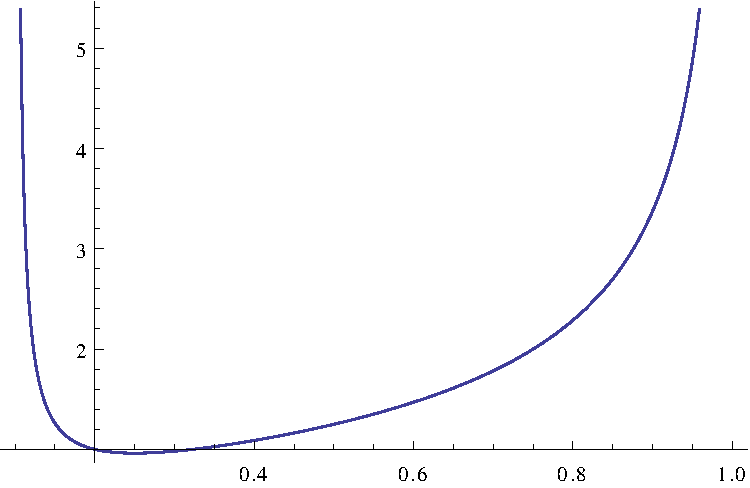
\includegraphics[width=.7\linewidth]{plot.pdf}
    \caption{%
        Integrand against $\rho$. The lower bound is chosen such that $\rho =
        \num{0.1}$. It can be seen that the integrand diverges at both bounds
        of integration.
    }
    \label{fig:plot.pdf}
\end{figure}

\subsubsection*{Restrictions on the domain}

If $\rho > f(\tS)$, this singularity does not occur. If $t < \tS$, this should
be given. The restrictions on the map are therefore
\[
    t < \tS
\]
so far.

Also $f(t)$ must not be greater than $1$ so that the integral does not return
negative values. Therefore $f(t) \leq 1$. Applying the inverse $f$ which is
bijective and strictly monotonically decreasing on the domain of interest, this
gives $t \geq 0$. The restrictions are now:
\[
    0 \leq t < \tS
\]

I can apply $f$ onto this restriction, paying attention to the flip in
direction. This gives me $f(0) \geq f(t) > f(\tS)$. I can then multiply that with
$r_0$ and get $r_0 f(0) \geq r_0 f(t) > r_0 f(\tS)$. Using the identities that
I have used previously, this becomes $r_0 \geq r > r_g$. Combined I get:
\[
    0 \leq t < \tS
    \quad\land\quad
    r_g < r \leq r_0
\]

The last restriction, $r_g < r f(t)$, is still missing.

\subsection*{(d) Mapping of the domain}

I will start off by looking at the corners of the domain.

\subsubsection*{Individual corners}

\paragraph{Corner $(r_g/f(0), 0)$}

The integral vanishes since $S$ becomes 1. The first corner gets transformed
to:
\[
    \del{\frac{r_g}{f(0)}, 0} \mapsto (r_g, 0)
\]

\paragraph{Corner $(r_g/f(\tS), \tS)$}

With this one, the integral diverges since $S$ becomes $f(\tS)$. Therefore, the
mapping of this corner is:
\[
    \del{\frac{r_g}{f(\tS)}, \tS} \mapsto (r_g, \infty)
\]

\paragraph{Corner $(r_0, 0)$}

\[
    (r_0, 0) \mapsto (r_0, 0)
\]

\paragraph{Corner $(r_0, \tS)$}

\[
    (r_0, \tS) \mapsto (r_g, \infty)
\]

\paragraph{Corners and restrictions}

Those four corners abide the restriction $0 \leq \bar t < \infty$ of the image
of the domain $D$, $\bar D$. The restriction $r_g \leq \bar r \leq r_0$ is
abided as well. It remains to be shown that the corners abide the remaining
$\bar r \leq r_0 f(t(\bar t))$ as well.

When $(\bar r, \bar t) = (r_g, 0)$, then the $f(t)$ in the $\bar t$ in the
implicit definition of $t$ has to be $1$, such that the integral vanishes.
Therefore, the restriction $\bar r \leq r_0 f(t(\bar t))$ simplifies to $r_g
\leq r_0$, which is satisfied.

When $(\bar r, \bar t) = (r_g, \infty)$, the $f(t)$ has to be $ar_0^2$, which
means that it is $r_g/r_0$. The restriction therefore is $r_g \leq r_g$,
which is also satisfied.

When $(\bar r, \bar t) = (r_0, 0)$, the restriction is $r_0 \leq r_0$, which is
also true.

\subsubsection*{Whole domain}

Since the mappings are diffeomorphisms, they need to be invertible. Since they
are invertible, they need to be bijective. Since they need to be continuous,
they need to be strictly monotonic. So I think I can conclude from the corners
that the interior is mapped properly.

\subsection*{(e) Conclusion about map}

I am supposed to conclude that we obtain a map $\tilde \phi \colon D \to \bar
D$ which satisfies $\tens g = \tilde \phi^* \tilde{\tens g}$.


The coordinates that are used in this problem are the Schwarzschild coordinates
which are called $\tens y$. Those are the ones with the bar on top, so I will
call this system $\bar \Sigma$. Then there are the comoving coordinates that
are $\tens x$ without any decoration, so I call the system $\Sigma$.

The quantity $\tilde{\tens g}$ looks odd at first. There is a $\bar{\tens g}$
defined in (12) on the problem set, and the metric in the comoving coordinates
$\tens g$ is given in (5). The metric $\tilde{\tens g}$ is defined in (18), and
it depends on the coordinates without any decoration explicitly in (18) and in
the definitions of $A$ and $B$ in (16). So I would assume that this metric
belongs to the system of comoving coordinates $\Sigma$.

The map $\tilde \phi$ maps from $D$ to $\bar D$, which also means that it maps
the coordinates $\Sigma$ to $\bar \Sigma$, i.\,e. it maps from the comoving
coordinates to the Schwarzschild coordinates.

In part (b) of this problem, I have attempted to show that equation (19) holds.
There, $\tens g$ is the image of $\tilde{\tens g}$ with a transformation that
maps from $\tens x$ to $\tens y$. This mapping maps from $\Sigma$ to $\bar
\Sigma$ and should therefore be $\tilde \psi$.

So what do I really have to conclude here? It cannot simply be that I have
proven this earlier, right?

The second part is to show that $\tilde{\tens g} = \bar{\tens g}$ holds when
$\bar r = r_0 f(t)$ and $\bar t = \bar t(r_0, t)$. That means that $r = r_0$
and $t = t$ in $\Sigma$. With the identities in equation (17) from the problem
set that I have shown in part (a), this is very easy, unless I overlooked
something.
\begin{align*}
    \bar g_{00} &= 1 - \frac{r_g}{\bar r}
    &
    \tilde g_{00}(t, r_0) &= 1 - \frac{r_g}{\bar r(t, r_0)} \\
    \bar g_{11} &= - \sbr{1 - \frac{r_g}{\bar r}}^{-1}
    &
    \tilde g_{11}(t, r_0) &= - \sbr{1 - \frac{r_g}{\bar r(t, r_0)}}^{-1} \\
    \bar g_{22} &= - \bar r^2
    &
    \tilde g_{22} &= - r^2 f(t)^2 \\
    \bar g_{33} &= - \bar r^2 \sin(\theta)^2
    &
    \tilde g_{33} &= r^2 f(t)^2 \sin(\theta)^2
\end{align*}
With $\bar r = r f(t)$, all the right sides are equal to the left sides. To the
two metrical tensors are equal at those given points.

Keeping $r_0$ fixed in the comoving coordinates means that we are inspecting
the immediate neighborhood of an observer that moves with the dust cloud. Time
just runs in the comoving coordinates, and it is mapped to $\bar t$
appropriately. I think this means that the metric at the edge of the cloud
looks the same to a comoving observer and a stationary observer outside the
Schwarzschild radius.

\IfFileExists{\bibliographyfile}{
    \printbibliography
}{}

\end{document}

% vim: spell spelllang=en tw=79
